% !TEX encoding = UTF-8
% !TEX TS-program = pdflatex
% !TEX root = ../tesi.tex

\newpage
\section{Design Pattern utilizzati}\label{sec:design-pattern-utilizzati}
Di seguito, sono elencati i design pattern utilizzati durante la creazione del tool. Per ognuno di questi, verrà fornito il diagramma delle classi e una descrizione.
\subsection*{Model View Controller}\label{subsec:model-view-controller}
Come pattern architetturale è stato adottato il pattern Model-View-Controller, poiché è in grado di separare la logica di presentazione dei dati dalla logica di business.\\
L'applicazione di tale pattern avviene attraverso il pattern Observer, nello specifico, le singole componenti della vista osservano i valori della classe Modello, in questo modo, quando il valore di un determinato attributo viene modificato, il nuovo valore viene notificato alla componente della vista.
\begin{figure}[H]
    \centering
    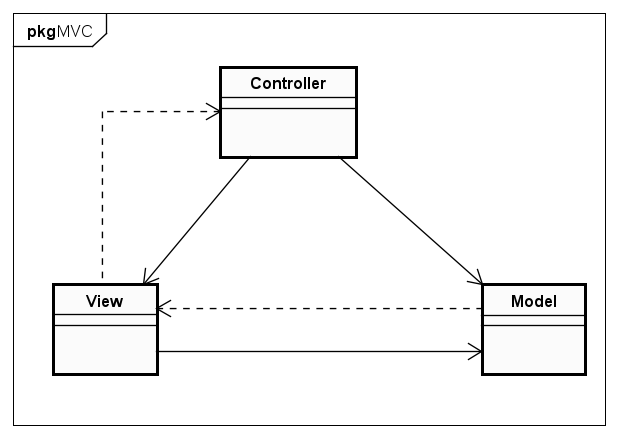
\includegraphics[width=13cm, height=8cm]{./immagini/diagrammi_uml/mvc.png}
    \caption{Diagramma delle classi del pattern MVC}\label{fig:mvc}
\end{figure}

\newpage
\subsection*{Observer}\label{subsec:observer}
Il pattern observer permette di definire una dipendenza uno a molti fra oggetti, in modo tale che se un oggetto cambia il suo stato, tutti gli oggetti dipendenti da questo siano notificati e aggiornati automaticamente.\\
Tale pattern viene applicato nel tool perché i componenti delle viste possano osservare il contenuto del modello.
\begin{figure}[H]
    \centering
    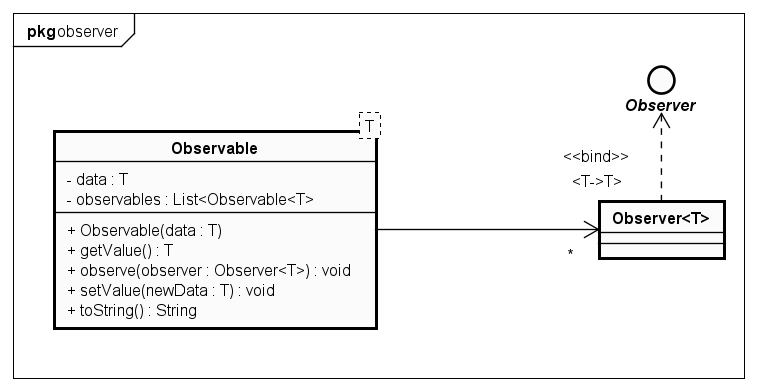
\includegraphics[width=13cm, height=8cm]{./immagini/diagrammi_uml/Observer.png}
    \caption{Diagramma delle classi del pattern Observer}\label{fig:observer}
\end{figure}

\newpage
\subsection*{Decorator}\label{subsec:decorator}
Il pattern decorator è stato utilizzato per creare la parte del tool che si occupa di effettuare l'analisi del codice decompilato e dei file scaricati dall'area di storage dell'applicazione presenti nell'Android Emulator Device.\\
Il vantaggio ottenuto per aver utilizzato questo pattern è quello di poter "decorare" l'oggetto base di analisi, ovvero l'istanza della classe \textit{BaseAnalyzer} con i vari decorator, un altro importante vantaggio è quello di poter aggiungere altre funzionalità di analisi facilmente nel tool, infatti, è sufficiente creare un'altra sottoclasse della classe \textit{BaseAnalyzeDecorator} quindi implementare il metodo astratto.
\begin{figure}[H]
    \centering
    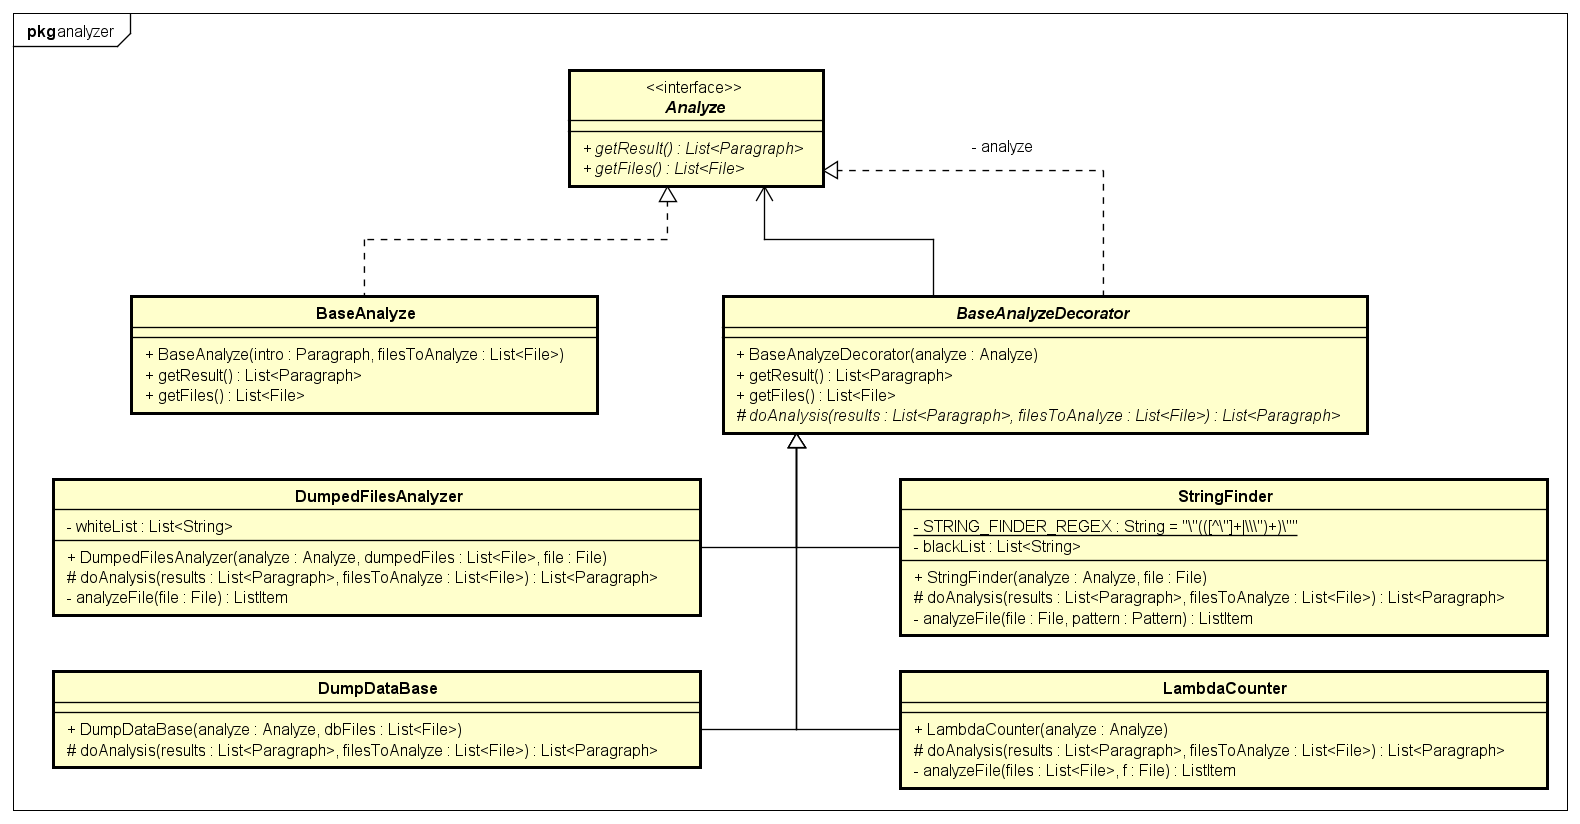
\includegraphics[width=13cm, height=10cm]{./immagini/diagrammi_uml/Decorator.png}
    \caption{Diagramma delle classi del pattern Decorator}\label{fig:decorator}
\end{figure}

\newpage
\subsection*{Factory Method}\label{subsec:factory-method}
Questo pattern è stato utilizzato per poter fornire al controller dei comandi da eseguire nei processi, essendo i comandi dipendente dal sistema operativo, sono state create due classi, una per Windows chiamata \textit{WindowsCommandFactory} e una per Linux chiamata \textit{LinuxCommandFactory}.
Allo start-up del tool, viene letta una dalla JVM una variabile chiamata \textit{os.name}, e dipendentemente da valore letto, viene deciso quale delle sottoclassi istanziare per il corretto funzionamento del tool.
\begin{figure}[H]
    \centering
    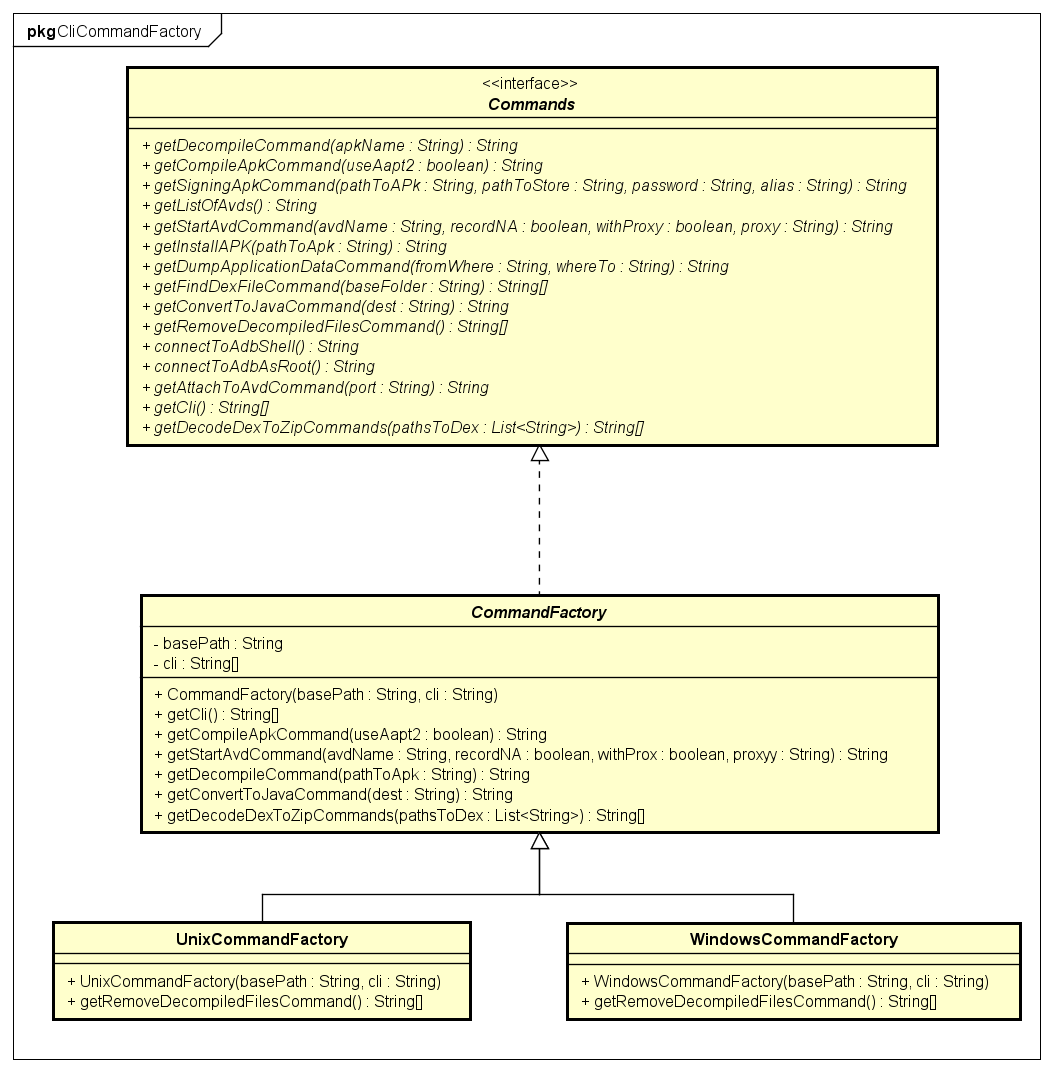
\includegraphics[width=14cm, height=12cm]{./immagini/diagrammi_uml/CommandFactory.png}
    \caption{Diagramma delle classi del pattern FactoryMethod}\label{fig:factory-method}
\end{figure}